\chapter{热类木星统计性质} \label{chapter:data_stat}

\section{系外行星统计列表}

在引言部分 \S \ref{sec: exopftheory},我们曾提到在如今已探测的系外行星中,有一群周期
小于十天却拥有大于土星质量的行星种群,被称为热类木星\footnote{若按照热类木星的定义,
其准确叫法应为近距离类木星,因为行星的有效温度不仅仅与主星的距离有关,而且还与主
星的有效温度有关。}。为了研究此类行星的统计性质,本文汇总了知名的四大系外行星数据
库网站 \url{http://exoplanets.eu/}、\url{http://exoplanets.org/}、\url{http://
exoplanetarchive.ipac.caltech.edu/} 和 \url{http://openexoplanetcatalogue.com/} ,并整理出
比较统一规范的系外行星列表\footnote{\url{https://github.com/EXONJU/ExoPlanetList}}。如
图 \ref{fig:hrplanet} 与 图 \ref{fig:exoskydist} 所示,在这行星数目为 3701 的样本中,共有 
375 颗系外热类木星系统(后文简称 HJs)。系外行星在南北天球分布并没有太多不均匀性
(除了巡天观测密集的几个区域以外),而 HJs 却在巨星分支中出现概率偏小(在 \S 
\ref{sec:hjofgiants} 中讨论),且大多数集中在类太阳恒星周围(下文介绍此为观测选择效
应)。本章节后续分析将统一建立在此 HJ 列表的范畴内讨论。

\begin{figure}
\centering
\includegraphics[width=1.0\textwidth]{figures/chapter4/fig2_HRplanet.pdf}
\caption{已确认系外行星的色指数与光度分布图,墨蓝色点为伊巴古星表临近太阳 150 pc 以内的恒星(图 \ref{fig:hrdiagram}),红五角星为太阳,绿色与黄色点如图 \ref{fig:exoskydist},被探测到的系外行星以及热木星明显集中在类太阳恒星附近,为观测选择效应。}
\label{fig:hrplanet}
\end{figure}


\begin{figure}
\centering
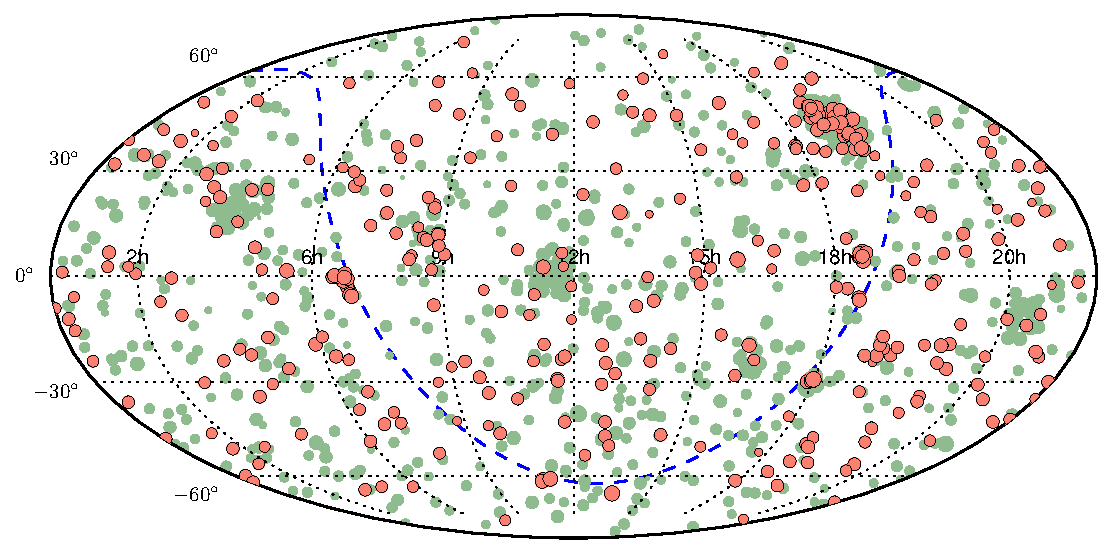
\includegraphics[width=1.0\textwidth]{figures/chapter4/fig1_exodistmollweide.pdf}
\caption{已被确认的系外行星在赤道坐标下的天球分布。图中蓝色虚线为银道面,可以看到巡天一般会远离银盘面(CoRoT 与 OGLE 除外)。绿色点为所有行星,黄色点则为热木星,点大小正比于 V 波段星等,从此图未见南北天的观测选择效应,$Kepler$ 视场(RA=19h 22m 40s,Dec=+44$^\circ$ 30' 00'' )为已确认系外行星最密集的区域之一。}
\label{fig:exoskydist}
\end{figure}


\section{HJs 出现概率}  \label{sec:hjoccurate}

按照已有的数据,现今探测到的 HJ 总数目约占已确认行星的 10\% 之多,这也是为什么
在图 \ref{fig:exomassper} 中,明显可以观察到一群质量在木星质量周期小于十天的行星
族。然而这与观测的选择效应密不可分。一个完备的统计必须建立在限定体积样本(
Volumn-limited sample)之上(文献 \citen{WinnFabrycky2015})。在一个限定体积的样
本中,热木星出现的概率并不高。Cumming 等人于 2008 年对 RV 巡天中的 600 颗 FKGM 
恒星监测了 8 年后的结果显示\cite{Cumming2008},对于 $M_\tif{p} > 100 \tif{M}_\oplus,\, 
P<5.5$ years 的行星的出现概率可用如下公式描述:

\begin{equation} \label{eq:pltoccurate}
\frac{\tif{d} N}{\tif{d}\ln M_\tif{p} \tif{d}\ln P} \propto  M_\tif{p}^\alpha P^\beta \ \, ,
\end{equation} %myequation{行星出现数目的概率分布}
其中指数 $\alpha = -0.31 \pm 0.20 $,$\beta = 0.26 \pm 0.10$。结合其他种类的巡天项目,
对应的 HJs 的出现概率大致为 0.5 \% 到1.5 \% 之间不等\cite{Howard2012,Marcy2005,
Mayor2011,Wright2012}。此概率的不同和恒星的星族选择密切相关\cite{Wright2012},比如
恒星的金属丰度和类木星出现的概率有明显的正相关性\cite{Gonzalez1997,Santos2001,
Santos2004,Fischer2005,Udry2007,Sozzetti2009,Sousa2011},这也恰好佐证了 \S 
\ref{sec:clspftheory} 中描述的气巨星重元素核吸积模型。


\section{HJs 形成} \label{sec:hjform}


在传统的核吸积模型中\cite{IdaLin2004b},气巨星往往需要在距离主星几个天文单位的地方
才能有足够多的原材料(绝大部分由冰组成)供固态核形成。然而在观测中,HJs 的统计
分布于 3 天附近存在峰值(见图 \ref{fig:hjperecc})。因此需要解释 HJ 的形成,大致上有
两大种方法:在传统的行星形成基础上引入木星的轨道迁移(\textit{orbital migration})或
直接于当地形成(\textit{in situ. formation})

\begin{figure}[t]
\centering
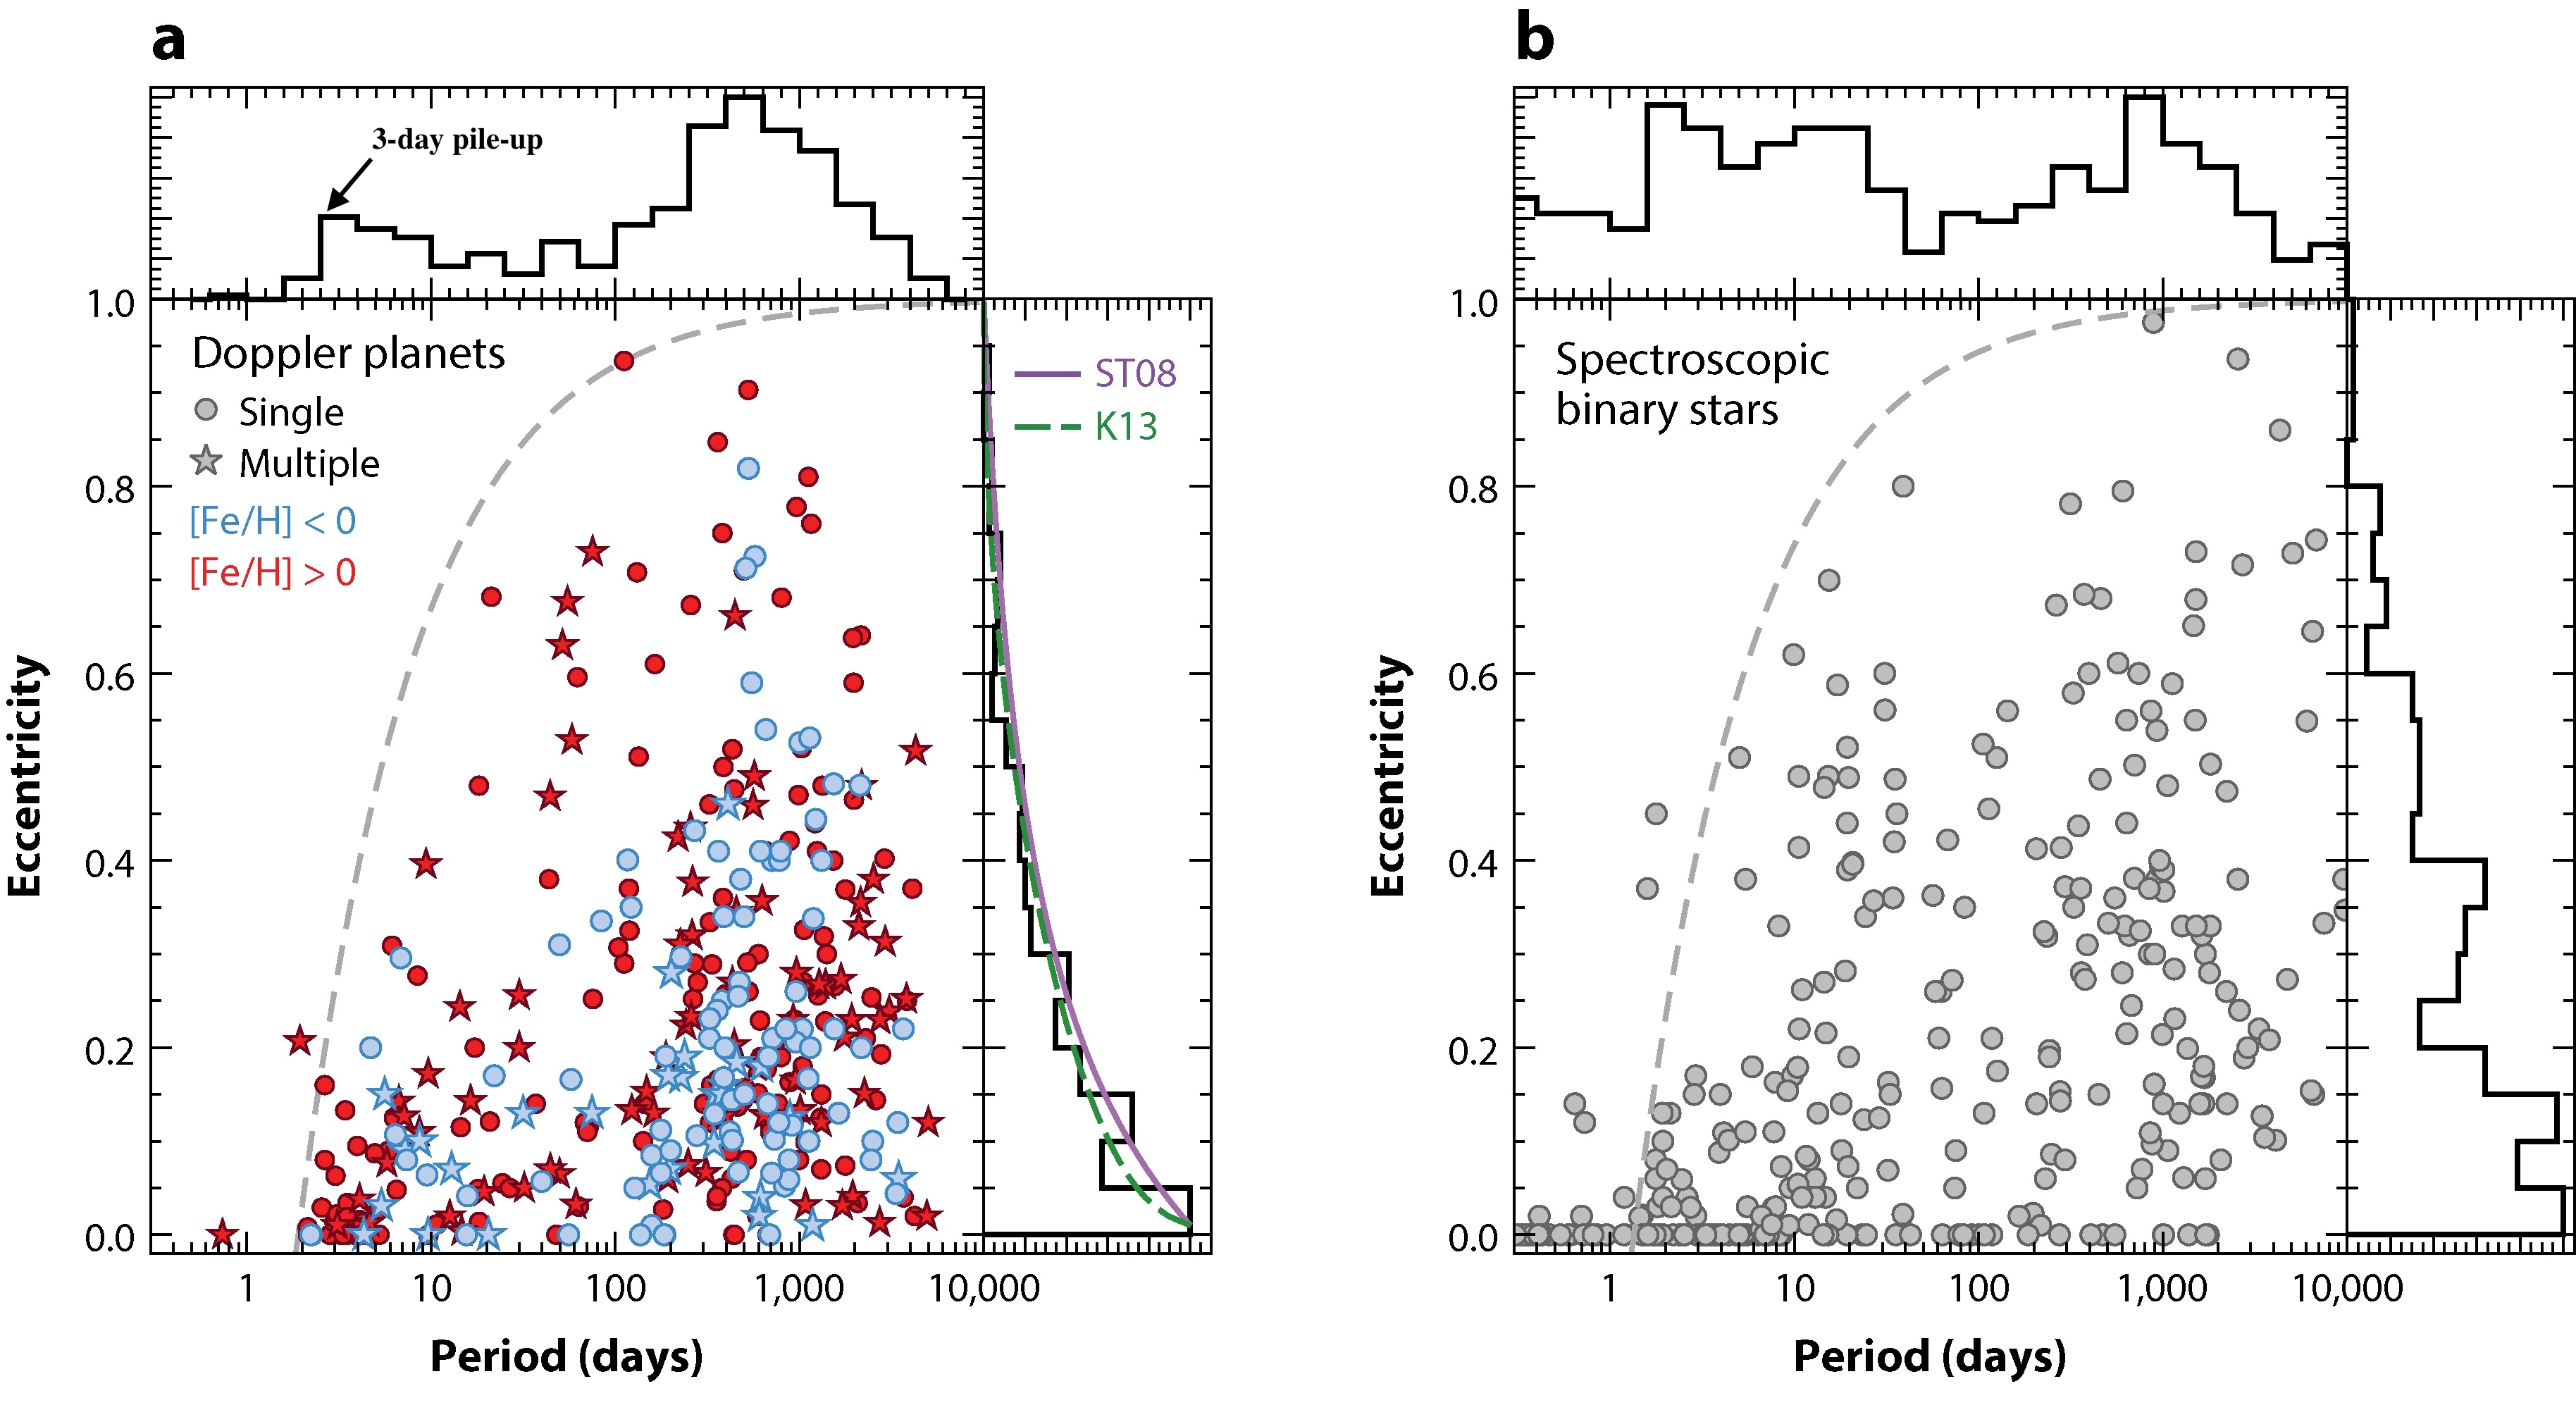
\includegraphics[width=1.0\textwidth]{figures/chapter4/fig3_peccdist.jpeg}
\caption[热类木星系统的周期与轨道偏心率分布图。可以看到系外行星样本(未经过选择效应修正)在三天周期分布达到热类木星的峰值,虚线为类太阳恒星周围行星拥有近心点距离 $a(1-e) = 0.03$ AU 的轨道。右侧图为 SB9 光谱双星星表的类似分布图,图片取自 Winn 和 Fabrycky。]{热类木星系统的周期与轨道偏心率分布图。图片取自文献 \citen{WinnFabrycky2015},可以看到系外行星样本(未经过选择效应修正)在三天周期分布达到热类木星的峰值,虚线为类太阳恒星周围行星拥有近心点距离 $a(1-e) = 0.03$ AU 的轨道。右侧图为 SB9 光谱双星星表的类似分布图。}
\label{fig:hjperecc}
\end{figure}


\subsection{轨道迁移}

在传统的行星形成的基础上,行星的轨道迁移并不需要引入额外的行星核心生长以及气体
吸积机制。轨道迁移代表着轨道半长径 $a$ 发生了变化,在椭圆二体运动中行星的角动
量与能量拥有如下表达式(本文内均假设 $M_\tif{p} \ll M_\tif{s}$):

\begin{equation} \label{eq:2be}
E = M_\tif{p}  \frac{\mu}{2a}
\end{equation} %\myequation{二体运动中的能量}

\begin{equation} \label{eq:2bam}
J = M_\tif{p} n a^2
\end{equation} %\myequation{二体运动中的角动量}
其中 $n$ 为平均轨道角速度,满足开普勒第三定律 $n^2a^3=\mu$,其中$\mu = G M_\tif{s}$
如此轨道迁移势必意味着角动量与能量的交换,因此必须有其它物体与行星之间发生角动量
与能量的传递与交换。这样一来,我们又可将轨道迁移大致分为两种情况:气体盘迁移(
\textit{disk migration})和高偏心率迁移(\textit{high-e migration})。

\subsubsection{气体盘迁移} \label{sec:diskmig}

由于木星质量的行星核心形成后会依然嵌套在恒星周围的气体盘内,因而由于盘的气体和之
间会存在角动量交换。这样的的角动量交换通常是通过 Lindblad 共振来实现\cite{Binney1987,
GoldreichTremaine1979},比如土星环\cite{GoldreichTremaine1980}。简单来说第 $m$ 阶共
振距离主星半径与行星轨道之间的关系为 $r_\tif{L} = (1\pm 1/m)^(2/3) a_\tif{p}$。在二体问
题中希尔半径(洛希半径)可描述为:

\begin{equation} \label{eq:hillradius}
r_H = \big( \frac{M_\tif{p}}{3M_\tif{s}} \big) ^{1/3}
\end{equation} %myequation{希尔半径(或洛希半径)表达式}

如果行星的质量足够大,使得希尔半径大于盘的标高($r_H > h$),那么盘可能被被打开缺
口。与此同时,由于气体盘的粘性,此缺口也可能被气体重新填上。1986 年,Lin 等人通过
比较盘缺口由于粘性重新被填补上以及由于 Lindblad 共振又再被打开的时标,得出在经典的
原行星盘参数下,木星质量的行星足够打开空缺,而土星的质量约为打开空缺的临界值
\cite{Lin1986,Ward1997},并且被成功地在人类发现的第一颗类太阳系外 HJ --- 51 Peg b 上
\cite{Lin1996},比如在 5 AU 附近的木星,在标准的行星盘打开缺口后,将在时标为 0.5 Myr 
左右迁移至原行星盘的内边界。这样的气体盘迁移又被称作第二型(Type II)轨道迁移(见
图 \ref{fig:diskmig})。

\begin{figure}[t]
\centering
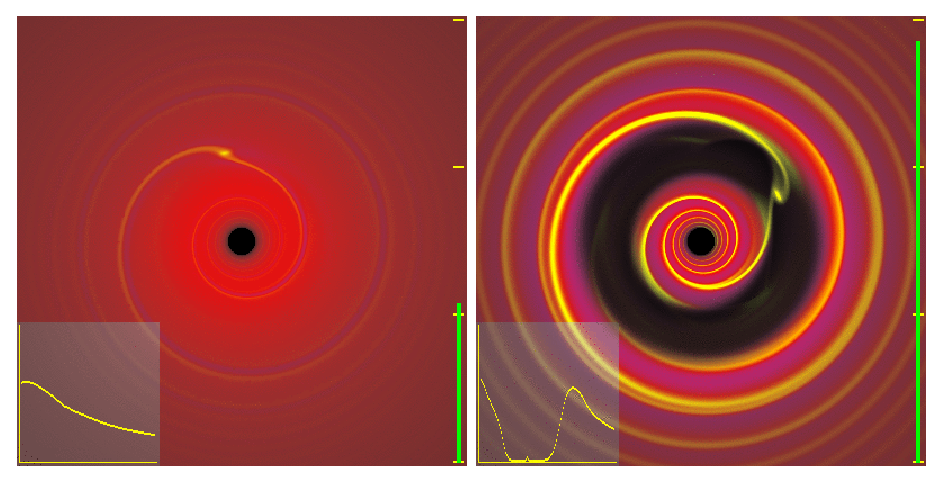
\includegraphics[width=1.0\textwidth]{figures/chapter4/fig3_diskmig.eps}
\caption[典型的第二型轨道迁移数值模拟,大质量行星可以在盘内打开空缺,并且往靠近恒星的盘内侧迁移。图片版权 Armitage\/Rice。]{典型的第二型轨道迁移数值模拟,大质量行星可以在盘内打开空缺,并且往靠近恒星的盘内侧迁移。图片取自文献 \citen{Armitage2005}。}
\label{fig:diskmig}
\end{figure}


\subsubsection{高偏心率迁移}






小质量的天体几乎不能改变木星

\textbf{Lidov-Kozai effect}

\textbf{planet-planet scattering}

\textbf{secular chaos}


\subsection{本地形成}




\section{恒星行星潮汐作用} \label{sec:spinteract}


\section{Holt Rossiter-McLaughlin 效应}
凌星 
统计样本
\url{http://www.astro.keele.ac.uk/jkt/tepcat/rossiter.html}


\section{热木星的自转轨道倾角与潮汐作用} 

\subsection{类太阳恒星}

星风

\subsection{中等质量恒星}

\subsection{讨论}




